\chapter{Urban Weather Generator}

\AddToShipoutPictureBG*{%
  \AtPageUpperLeft{%
    \hspace*{18.35cm}%
    \raisebox{-3cm}{%
      \makebox[0pt][r]{\parbox{\textwidth}{\begin{flushright}\textit{``All models are wrong, but some are useful.''}\\
      George Box\end{flushright}}}
}}}%

In order to capture the UHI effect and to simulate the microclimate condition, the Urban Weather Generator (UWG) was developed by Bueno et al. \cite{bueno2013urban} as a stand-alone program to map a reference weather file to the estimated conditions at a neighborhood scale based on the specific urban area characteristics.

\section{Program introduction}

The wisdom of UWG comes from the fact that many communities do not have access to the microclimate information from local experimental measurements and mesoscale simulation results, while the rural meteorological information can be easily found in currently available weather files. Starting with the rural weather data provided in the EPW format and the urban characteristics, the UWG outputs the simulated urban weather data (during either an entire calendar year or just a subset thereof) that can be readily used in the EPW format.

\begin{figure}
\centering
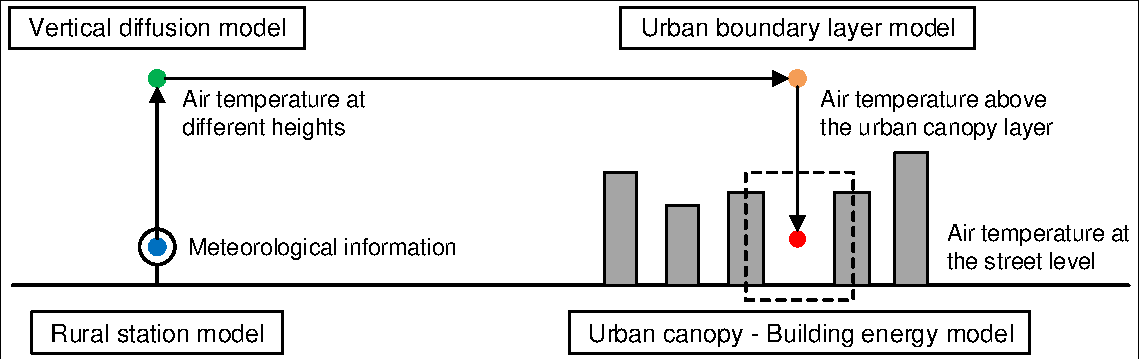
\includegraphics[width=.8\linewidth,trim=2 2 2 2,clip]{UWG.pdf}
\caption{Four coupled models in the UWG (mainly from Ref. \cite{bueno2013urban}).}
\end{figure}

As shown in \textbf{Figure 2-1}, the UWG consists of four coupled models: the rural station model (RSM), the vertical diffusion model (VDM), the urban boundary layer model (UBLM), and the urban canopy-building energy model (UC-BEM). Detailed physical mechanisms of these models can be found in Refs. \cite{bueno2013urban, bueno2013calculation}. Originally written in \textsc{Matlab}, following update of the UWG program further includes XML \cite{nakano2015urban} and Excel \cite{yang2016curious} interfaces to allow flexibility in input formats of the urban characteristics. General workflow of the UWG program is depicted in \textbf{Figure 2-2}. The version used in this thesis is a macro-enabled Excel interface along with compiled \textsc{Matlab} scripts of the UWG as a standalone urban microclimate simulation package.

\begin{figure}
\centering
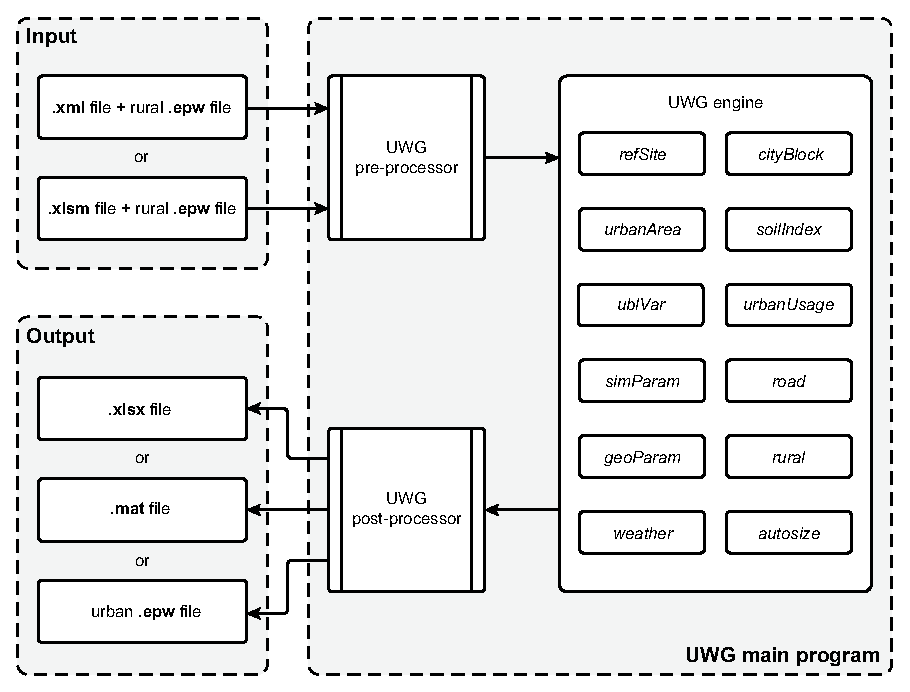
\includegraphics[width=.825\linewidth]{UWGEngine.eps}
\caption{General workflow of the UWG program (mainly from Ref. \cite{yang2016curious}).}
\end{figure}

Based on the main UWG code, \textsc{Dragonfly} is a new component for Grasshopper and Rhino that allows users to model and estimate large-scale climate phenomena, such as the UHI effect. This is accomplished with the help of several urban thermal simulation engines, including the UWG and CitySim \cite{robinson2009citysim}. It also links to several climate-related datasets such as the Hadley Global Circulation Model (for climate change projections) and to several satellite image datasets such as the Landset and MODIS from NASA. The \textsc{Dragonfly} program intends to make many large-scale climate variables accessible to the visual scripting interface of Grasshopper as well as the 3D visualization interface of Rhino. The latest executable tool and program code (in Python) are currently maintained by Mackey et al. \cite{mackey2015dragonfly} on GitHub.

\section{Program update}

Since the previous version in 2014 \cite{bueno2014computationally}, the UWG has been updated in 2016 \cite{yang2016curious}, especially for the urban boundary layer model and the urban canopy-building energy model, with the purpose of making it more physically sound and more capable to handle increasingly detailed building definition. Major updated features of the current UWG are re-emphasized and described below.

\subsection{Urban canopy model}

Based on the Town Energy Balance (TEB) scheme proposed by Masson \cite{masson2000physically}, the UWG maps the 3D urban geometry to a 2D canyon model consisting of a wall, roof, and road, representative of the average urban characteristics. While the previous version bounded the canyon volume by twice the building height, the urban boundary layer (UBL) in the new version extends down to the top of the building. All heat released from the roof is assumed to directly enter the UBL. This makes the formulation more consistent with the original TEB scheme.

The direct solar radiation in the new version is also updated for numerical stability. According to Masson \cite{masson2000physically}, their fractions are given by:

\begin{equation}
K_{w,dir}=\min \Bigl\{ \frac{w_r}{h_{bld}} (\frac{1}{2} - \frac{\theta_0}{\pi}) + \frac{1}{\pi} \tan (\lambda)(1 - \cos (\theta_0)),\; 1 \Bigr\}\,,
\end{equation}

\begin{equation}
K_{r,dir}=\min \Bigl\{ \frac{2\theta_0}{\pi} - \frac{2}{\pi} \frac{h_{bld}}{w_r} \tan (\lambda)(1 - \cos (\theta_0)),\; 1 - 2 r_{aspect} K_{w,dir} \Bigr\}\,,
\end{equation}

\vspace{15pt}
\noindent where $K_{w,dir}$ is capped to 1 as the sun approaches the horizon.

While Masson defined these terms to scale the direct solar radiation received by a horizontal surface, the value specified in a standard EPW file is the direct normal radiation, namely the solar radiation received by a surface perpendicular to the sunlight direction. This indicates that the previous model had a slightly excessive solar gain. Thus, the direct solar radiation in the newest UWG is modified as:
\vspace{12pt}
\begin{equation}
S_{hor,dir} = S_{norm,dir} \cos (\lambda)\,.
\end{equation}

\vspace{9pt}
In terms of the infrared radiation (IR) exchange, the previous version seemed to over-estimate the IR absorption by bodies of air \cite{fenn1985optical}. To correct this over-estimation, the air is now assumed to be essentially transparent to the long-wavelength (LW) radiation emitted from its boundary surfaces. This assumption has been validated with MODTRAN simulations \cite{yang2016curious}, showing that the IR absorption of the air is almost negligible for the thick air bodies (around 1 km) considered in the UWG. Thus, the net LW heat exchanges with the atmosphere for the roof, wall, and road are given as:

\begin{equation}
Q_{LW,roof} = \epsilon_{roof} (Q_{LW,down} - \sigma T^4_{roof})\,,
\end{equation}
\vspace{-1em}
\begin{equation}
\begin{split}
\hspace{-1.5pt} Q_{LW,wall} & = \epsilon_{wall} VF_{wall-sky} (Q_{LW,down} - \sigma T^4_{wall}) \\
& \hspace{12pt}+\hspace{3pt} \sigma \epsilon_{road} \epsilon_{wall} VF_{wall-road} (1 - r_{shade}) (T^4_{road} - T^4_{wall})\,,
\end{split}
\end{equation}
\vspace{-0.25em}
\begin{equation}
\begin{split}
\hspace{-1.5pt} Q_{LW,road} & = \epsilon_{road} VF_{road-sky} (1 - r_{shade}) (Q_{LW,down} - \sigma T^4_{road}) \\
& \hspace{12pt}+\hspace{3pt} \sigma \epsilon_{road} \epsilon_{wall} VF_{road-wall} (1 - r_{shade}) (T^4_{wall} - T^4_{road})\,,
\end{split}
\end{equation}

\vspace{21pt}
\noindent where $Q_{LW,down}$ has accounted for the radiative effect due to the water vapor and carbon dioxide contained in the UBL.

Since the latent heat exchange between the four coupled models was not fully considered, Yang \cite{yang2016curious} decided to remove the humidity calculation for canyon in the new version of UWG. This calculation requires consideration of the moisture from vegetation, soil, combustion, nearby bodies of water, etc., and these components have not been precisely modeled in the current UWG. It is also worth noting that the latent heat balance in the urban canyon has not been formally validated \cite{bueno2013urban,bueno2014computationally}. Thus, the absolute humidity in the rural area is assumed the same as that in the urban area, and is then used to calculate the relative humidity for the generated EPW file. When accounting for the solar radiation received by the vegetation, we only consider its sensible portion in the energy balance, subtracting a prescribed latent-energy fraction.

When the urban weather file is generated, the calculated canyon wind speed is included, instead of the rural wind speed used by previous versions. The calculation is detailed in the appendixes of Refs. \cite{bueno2013urban,bueno2014computationally}. In addition, the new UWG incorporates a user-specified hourly schedule for the traffic-generated heat flux, as a counterpart to the schedules defined in the building energy model, to make the simulated diurnal microclimate profile more accurate. Finally, the new version of UWG reads the soil temperatures from the EPW file, and uses these values as the boundary condition to obtain the road layer temperature profile. It is also worth noting that the road elements in the new version are divided into thinner layers (with maximum of 5 cm) so that the surface temperature fluctuation can be captured more precisely.

\subsection{Urban boundary layer model}

The urban boundary layer (UBL) model solves an energy balance for a control volume above the urban canopy layer (UCL) where the boundary conditions can be imposed \cite{bueno2013calculation}. The UBL is considered as a region of well-mixed and isothermal air below a capping inversion.

As explained in \textbf{Subsection 2.2.1}, the IR portion of the energy exchange added in 2014 \cite{bueno2014computationally} is now removed. Thus, the energy balance of the current UBL model remains the same as the original version in 2012 \cite{bueno2013calculation}, defined as:

\begin{equation}
V_{CV} \rho c_v \frac{d\theta_u}{dt} = H_u + \int u_{ref} \rho c_p (\theta_{ref} - \theta_u) dA_f\,,
\end{equation}

\vspace{15pt}
\noindent where the term on the LHS stands for the thermal inertia of the control volume, and the second term on the RHS stands for the advection effect.

The heat exchange at top of the control volume is assumed negligible when the vertical profile of the potential temperature provided by the vertical diffusion model is constant. So, the energy balance of the UBL model is driven only by the heat flux from the bottom or the lateral sides of the volume surface.

The advection effect is driven by either the horizontal flow or the radial urban-breeze circulation where the wind direction is not taken into account. Therefore, the rural weather data seems applicable to large concentric regions surrounding the urban area \cite{hidalgo2010scaling}.


\subsection{Building energy model}

The building energy model approximates the heat balance of the indoor air temperature for each building. For simplicity, the air temperature is assumed uniform within the entire building envelope. As a result, the UWG can capture the building energy operations and calculate the waste heat emissions from HVAC systems, which are the potentially significant sources of heat in the energy balance of an urban canyon.

Whereas the old version only specified the total internal heat load in buildings, the new UWG takes into account the variation in the types of heat loads. As shown in \textbf{Table 2.1}, the updated UWG treats the convective, latent, and radiant heat loads separately. The convective and latent heat exchange is added directly into the indoor air heat balance, while the radiant heat flux is received by the ceiling and floor. The view factors from lights and occupants to the ceiling and floor are assumed close to unity.

\begin{table}[]
\centering
\footnotesize
\caption{Fractions of the internal heat loads.}
\label{my-label}
\begin{tabular}{lllll}
\toprule
                    & Occupancy load & Equipment load & Lighting load & Added to \\ \hline
Convective fraction & 0.5            & 0.5            & 0.3           & Air      \\
Latent fraction     & 0.3            & 0              & 0             & Air      \\
Radiant fraction    & 0.2            & 0.5            & 0.7           & Mass     \\
\bottomrule
\end{tabular}
\vspace{2.5ex}

\raggedright Note: The fraction values are selected based on ASHRAE Handbook -- Fundamentals \cite{handbook2009american}.
\end{table}

To simplify the estimation of various building types at the neighborhood scale, commercial building reference data is imported from the US DOE online database \cite{deru2011us} into a spreadsheet associated with UWG. This allows the users to specify the building types that make up the urban area, instead of modeling all the buildings individually. Accordingly, the updated UWG simulates the hourly schedules of occupancy, lighting, and equipment loads for each building type using the default values provided in the DOE reference building database, with flexible options for user customization. The goal is a better estimation of the building energy use pattern at the urban scale and the temporal sensible heat fluxes released into the surrounding environment. In addition, we consider a single building zone with a generic thermal mass and use the multi-zone-weighted average to calculate the internal heat gain. The simplified building models have been validated against the original models in Ref. \cite{yang2016curious}.

For the heating mechanism in the updated version, the internal heat gain is added into the building control volume based on the heating requirement, instead of based on the supply air temperature and mass flow rate. On the other hand, the cooling demand is determined by a psychrometric model based on the apparatus dew point. If the energy demand is greater than the system capacity, the system capacity is then used to calculate the supply air temperature.

In order to properly size the building elements, detailed information for the case study is determined according to local summaries and then is substituted into the DOE reference building database. As for the thermal properties of the building envelope, if the insulation layer is too thin (less than 1 cm), it will not be modeled in the structural element to avoid solver instability. Such omission will not significantly affect the thermal characteristics of the structure. However, the surface optical properties, such as the albedo and emissivity, are still taken into account.

Finally, while the previous version calculated the waste heat based on the total building energy consumption, the updated version treats the waste heat in more detail. The energy consumed by lights and equipment is considered as the heat flux received by either indoor air or internal surfaces, eventually merging with the canyon air through windows and walls. The waste heat added directly into the canyon is calculated based on the HVAC-related waste heat (with a predetermined fraction), as well as the waste heat from hot water usage and gas consumption\footnote{Assuming that the zones where gas equipment is used are well-ventilated (indicated by exhaust rate for EnergyPlus models), the heat loads of gas equipment are not included in the internal sensible heat loads \cite{yang2016curious}. Hence, similar to space and water heating, a specified fraction of the gas consumption is added to the waste heat from the building(s).}.

